\documentclass[12pt]{article}

% Import packages
\usepackage{listings}  % For adding C++ code
\usepackage{xcolor}    % For custom colors
\usepackage{graphicx}  % For including images
\usepackage{amsmath}   % For advanced math formatting
\usepackage{hyperref}  % For creating hyperlinks
\usepackage{geometry}  % To set page margins
\usepackage{subfig}
\usepackage{float}
\geometry{a4paper, margin=1in}

\lstdefinestyle{cppstyle}{
    language=C++,
    basicstyle=\ttfamily\footnotesize, % Font style
    keywordstyle=\color{purple}\bfseries, % Keywords in blue
    stringstyle=\color{orange}, % Strings in red
    commentstyle=\color{olive}, % Comments in gray
    numbers=none, % No line numbers
    tabsize=4, % Tab space width
    showspaces=false,
    showstringspaces=false,
    frame=single, % Adds a single-line box around the code
    framerule=0.8pt, % Thickness of the frame
    framesep=5pt, % Space between frame and code
}

\title{\textbf{ESPX - Assignment 1}}
\author{Savvas Tzanetis - 10889}
\date{May 2025}

\begin{document}

\maketitle

\section{Preperations}
This report is part of the first assignment for the \textbf{Real Time Embedded Systems} class of the \textbf{Electrical and Computer Engineering} department at the \textbf{Aristotle University of Thessaloniki}.

\paragraph{}
The task of this assignment was to modify an existing implementation the \textit{Consumer-Producer Problem} written in the \textbf{C} programming language, in order to produce "work functions" that the consumer threads must execute. \\
More specifically, the modified codes producer threads parse to the shared queue work functions that compute the sin of a set of \textit{10} angles that are also parsed to the queue as function arguments.

\section{Results Evaluation}
Using \textbf{gettimeofday()}, we record the time that a \textit{work function} is added to the queue from the producer thread, as well as the time the same function is removed from the queue from a consumer. The results are gathered using 10 or 20 producer threads with a varying amount of consumer threads.

\begin{figure}[!h]
    \centering
    \begin{minipage}{0.48\textwidth}
        \centering
        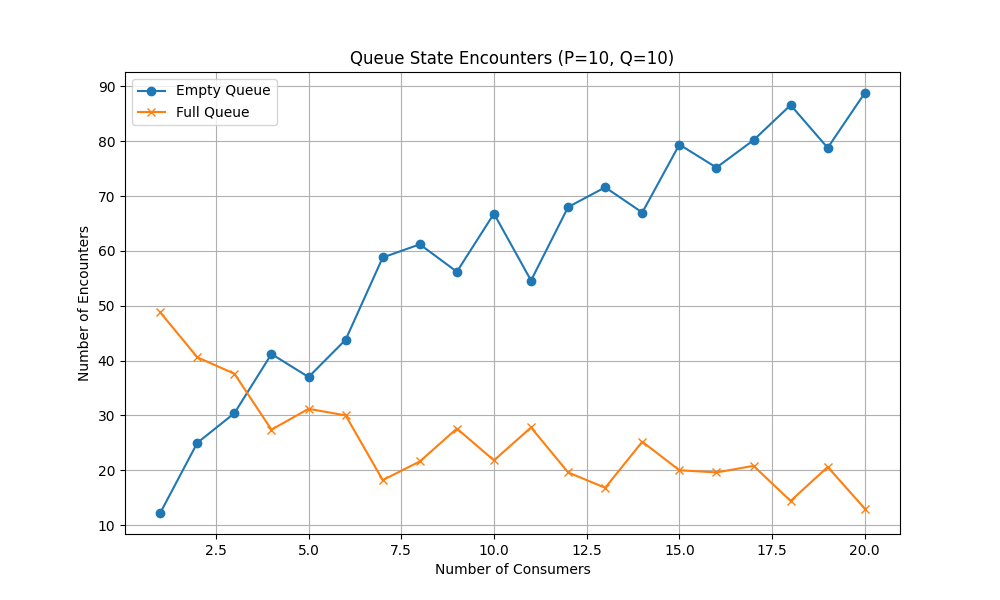
\includegraphics[width=\linewidth]{queue_state_p10_q10.png}
        \caption{Queue state with 10 producers}
        \label{fig:queue-p10}
    \end{minipage}%
    \hfill
    \begin{minipage}{0.48\textwidth}
        \centering
        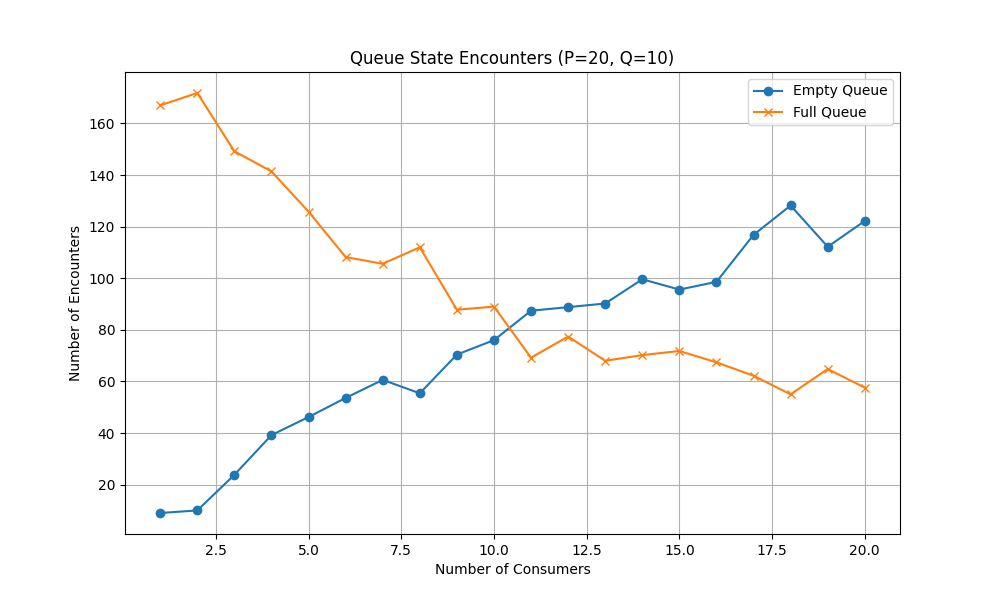
\includegraphics[width=\linewidth]{queue_state_p20_q10.png}
        \caption{Queue state with 20 producers}
        \label{fig:queue-p20}
    \end{minipage}
\end{figure}

\newpage
\begin{figure}[!h]
    \centering
    \begin{minipage}{0.48\textwidth}
        \centering
        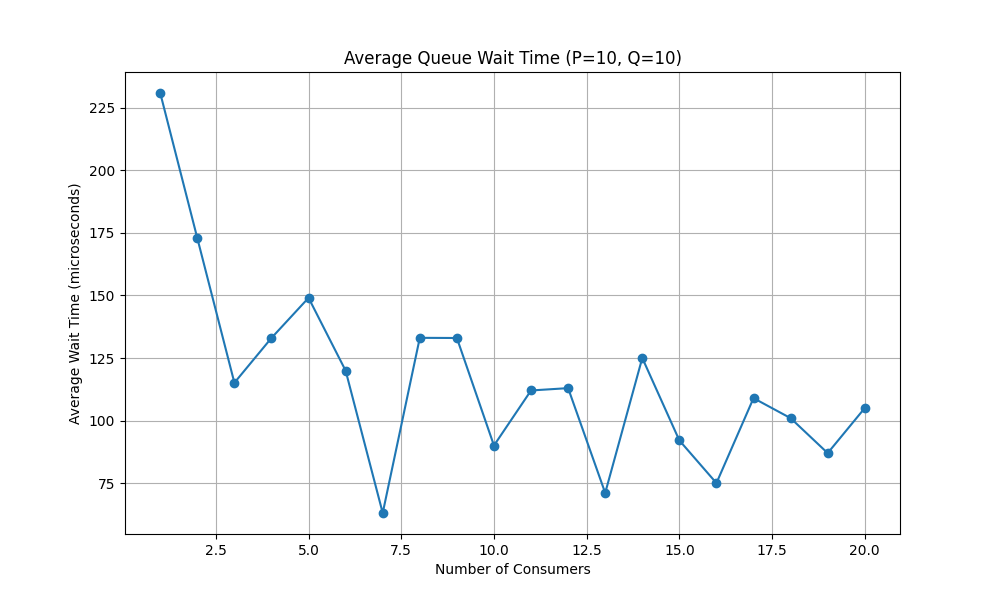
\includegraphics[width=\linewidth]{avg_wait_p10_q10.png}
        \caption{Average waiting time with 10 producers}
        \label{fig:queue-p10}
    \end{minipage}%
    \hfill
    \begin{minipage}{0.48\textwidth}
        \centering
        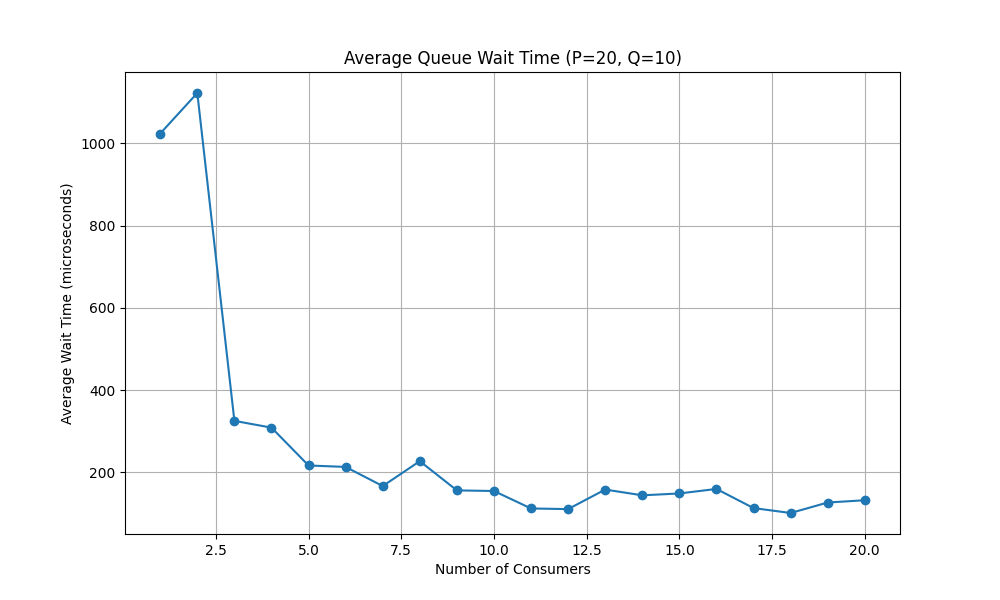
\includegraphics[width=\linewidth]{avg_wait_p20_q10.png}
        \caption{Average waiting time with 20 producers}
        \label{fig:queue-p20}
    \end{minipage}
\end{figure}

\subsection{Results Analysis}
Analyzing the presented figures reveals several key insights into the performance characteristics of our producer-consumer implementation.

\paragraph{}
In figures \textbf{1} and \textbf{2}, we show the queue state statistics with 10 and 20 producers respectively. In both scenarios, we find that the frequency of contacts with an empty queue increases continuously as the number of consumer threads increases.  The trend gets more noticeable when 20 producers are used.  Encounters in the full queue begin much higher and decline more gradually.

\paragraph{}
Figures \textbf{3} and \textbf{4} shows us expected results, revealing the relationship between consumer and producer thread count. With 10 producers, the average wait time shows an overall declining trend as consumer threads increase, with notable variability that could be suggesting diminishing returns and potentially increased scheduling overhead, while with 20 producers, we can observe significantly higher overall wait times, particularly with fewer consumers, while also dropping wait times more dramatically as more consumers are added.

\paragraph{}
These results provide practical guidelines for tuning thread counts in producer-consumer systems:
\begin{itemize}
    \item For optimal performance with fixed queue sizes, consumer threads should typically be close to equal to the number of producer threads.
    \item Systems should avoid extreme imbalances between producer and consumer threads, as these lead to either queue saturation or resource wastage.
\end{itemize}

\subsection{System Specifications}
The evaluation results where produced on a \textbf{Windows 11} machine with the following specifications:
\begin{itemize}
    \item \textbf{6-Core} Intel Core i5 CPU with \textbf{hyper-threading} running at \textbf{2.4Ghz}
    \item \textbf{16GB} RAM
\end{itemize}

\end{document}
